\lecture[2022-05-21]{Pandas II: Grouping, Aggregation, Pivot Tables Merging}

\subsection{Adding, Modifying, and Removing Columns}
Previously, we saw how we could find the most popular male names in California using \mintinline{text}{query} and sorting the result.

\begin{minted}{python}
babynames.query("Sex ==M and Year == 2020").sort_values("Count", ascending=False) # chooses only rows from 2020 which are male, then sort in descending order
\end{minted}

\begin{figure}[ht]
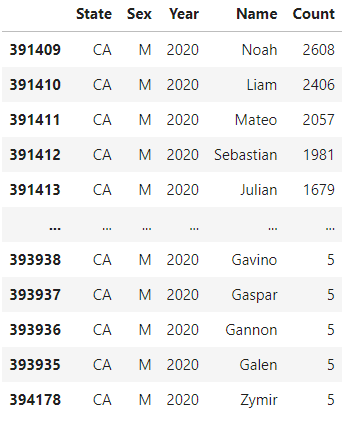
\includegraphics[width=0.4\textwidth]{4-sort1.png}\centering
\end{figure}

However, how can we find the longest names? If we sort by the names column, it will just return the names in reverse alphabetical order. After some searching, it turns out you can add in a \mintinline{text}{key} parameter which tells Pandas how to sort the values in the column.

\begin{minted}{python}
# start process - sorts names by alphabetical order
babynames.query("Sex == M and Year == 2020").sort_values("Name", ascending=False)
# new code - add key of baby name length
babynames.query("Sex == M and Year == 2020").sort_values("Name", key=lambda name: name.str.len(), ascending=False)
\end{minted}

\begin{figure}[ht]
\begin{minipage}{0.5\textwidth}
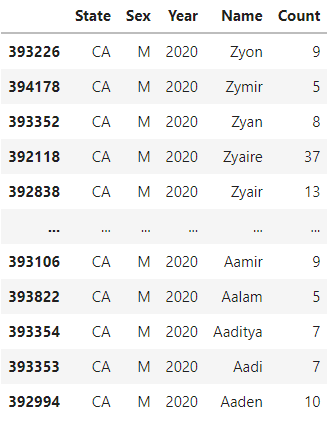
\includegraphics[width=0.65\textwidth]{4-sort2.png}\centering
\end{minipage}
\begin{minipage}{0.5\textwidth}
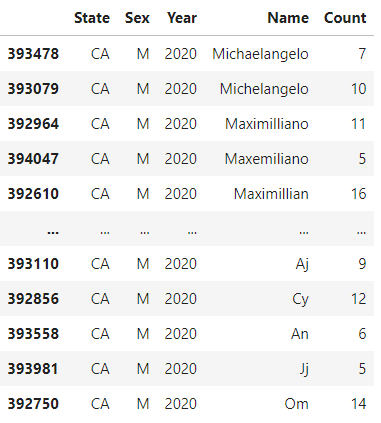
\includegraphics[width=0.65\textwidth]{4-sort3.png}\centering
\end{minipage}
\caption{The first approach only yields the names in reverse alphabetical order, but sorting with the \mintinline{text}{key} parameter yields the desired result.}
\end{figure}

However, this wasn't a feature until 2020. Prior to that, we would need to come up with another solution: 
\begin{itemize}
\item Create a temporary column getting the length of the baby name.
\begin{itemize}
\item Create a new series with only lengths.
\item Add the series to the dataframe.
\end{itemize}
\item Sort using that column.
\item Drop the temporary column. (General Form: \mintinline{text}{df.drop(<name>, (axis="columns"))})
\end{itemize}

\begin{minted}{python}
# creating a new column 
babynames["name_lengths"] = babynames["Name"].str.len() # new series - applies len to the Name series, then assigns the series "name_lengths" to the dataframe as a column
babynames = babynames.sort("name_lengths", ascending=False) # sort by name_length columns in descending order
babynames = babynames.drop("name_lengths", axis="columns") # drop the column - add axis = "columns" to specify it is a column (default drop rows)
\end{minted}

\subsubsection{Sorting by Arbitrary Functions}
To sort by arbitrary functions (e.g. \# occurrences of ``dr'' and ``ea'' in a string), use \mintinline{text}{Series.map} method. (Think of the \mintinline{text}{tbl.apply()} method in datascience)

\begin{minted}{python}
def dr_ea_count(string):
    return string.count("dr") + string.count("ea")

babynames["dr_ea_count"] = babynames["Name"].map(dr_ea_count) # Series.map(<func>)
babynames.sort_values("dr_ea_count", ascending=False)
\end{minted}
\begin{figure}[ht]
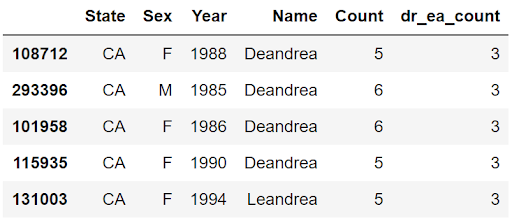
\includegraphics[width=0.5\textwidth]{4-map.png}\centering
\end{figure}

\subsection{Group By}
Let's try to find the female baby name whose popularity has fallen the most using RTP (ratio to peak - current number over peak number in a year).

e.g. for the name ``Jennifer'' measured in 2020, there were 172 Jennifers over the peak of 6064 Jennifers in 1972. Therefore, the RTP is $\frac{172}{6064} = 0.0233$.
\begin{figure}[ht]
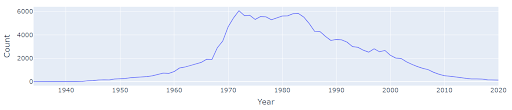
\includegraphics[width=0.75\textwidth]{4-rtp.png}\centering\caption{Graph of the amount of Jennifers each year.}
\end{figure}

Here's how to do it in Pandas:
\begin{minted}{python}
max_j = max(babynames.query("Name == 'Jennifer' and Sex == 'F'")["Count"]) # max on the count series based on the query (females born named Jennifer)
cur_j = babynames.query("Name == 'Jennifer' and Sex == 'F'")["Count"].iloc[-1] # same query, select count series, choose the last row
rtp = cur_j / max_j # find the rtp - current vs max

# simplifying
def ratio_to_peak(series):
    return series.iloc[-1] / max(series) # current / max 

j_counts = babynames.query("Name == Jennifer and Sex == 'F'")["Count"]
ratio_to_peak(j_counts) # returns the same results as the rtp variable 
\end{minted}

What about finding the RTP for every name and not Jennifer? A possible way is to create a dictionary of RTPs and get the RTP for each unique name.
\begin{minted}{python}
#build dictionary where each entry is the rtp for a given name, e.g. rtps["jennifer"] should be 0.0231
rtps = {}
for name in babynames["Name"].unique(): # use Series.unique to get an array of unique values in a series
    counts_of_current_name = female_babynames[female_babynames["Name"] == name]["Count"] # choose the rows corresponding to the correct name
    rtps[name] = ratio_to_peak(counts_of_current_name)

#convert to series
rtps = pd.Series(rtps)
\end{minted}
However, this approach is very slow and more complicated. The next method takes advantage of \mintinline{text}{.groupby} and \mintinline{text}{.agg}.

\begin{minted}{python}
female_babynames.groupby("Name").agg(ratio_to_peak) # group by column Name, aggregate through the rtp function
# data 8 approach 
female_babynames.group("Name", ratio_to_peak)
\end{minted}

\begin{notebox}[]
The second method (using \mintinline{text}{.groupby} and the Pandas API) is preferred and the one you should be using - you should never be writing code with loops or list comprehensions on Series.
\end{notebox}



\subsection{Pivot Tables}

\subsection{Joining Tables}



